% !TEX program = pdflatex
\documentclass[a4paper,12pt]{article}
\usepackage[utf8]{inputenc}
\usepackage[T2A]{fontenc} 
\usepackage[russian]{babel}
\usepackage{amsmath}
\usepackage{amssymb}
\usepackage{graphicx} % Пакет для вставки графики
\usepackage{listings}
\usepackage{booktabs}
\usepackage{geometry}
\usepackage{indentfirst}
\usepackage{xcolor}
\usepackage[hidelinks]{hyperref}
\usepackage{float}
\usepackage{indentfirst}
\usepackage{setspace}
\usepackage{tikz}
\usetikzlibrary{shapes.geometric, arrows.meta, positioning, calc}

\geometry{top=20mm,bottom=20mm,left=30mm,right=15mm}

\tikzset{
  startstop/.style={rectangle, rounded corners=8pt, minimum width=3.2cm,
    minimum height=0.8cm, draw=black, fill=gray!20, text centered, font=\small},
  process/.style={rectangle, minimum width=3.8cm, minimum height=0.8cm,
    draw=black, fill=white, text centered, font=\small},
  decision/.style={diamond, aspect=2.5, minimum width=4cm, minimum height=0.9cm,
    draw=black, fill=white, text centered, font=\small, inner sep=1pt},
  io/.style={trapezium, trapezium left angle=70, trapezium right angle=110,
    minimum width=3.4cm, minimum height=0.8cm, draw=black, fill=white,
    text centered, font=\small},
  arrow/.style={-{Stealth[length=6pt]}, thick}
}

\definecolor{codebg}{rgb}{0.95,0.95,0.95}
\definecolor{keywordcolor}{rgb}{0.0,0.0,0.55}
\definecolor{commentcolor}{rgb}{0.4,0.4,0.4}
\definecolor{stringcolor}{rgb}{0.55,0.0,0.0}

\lstdefinestyle{cppstyle}{
    language=C++,
    backgroundcolor=\color{codebg},
    frame=single, rulecolor=\color{gray!60},
    basicstyle=\ttfamily\small,
    keywordstyle=\color{keywordcolor}\bfseries,
    commentstyle=\color{commentcolor}\itshape,
    stringstyle=\color{stringcolor},
    numbers=left, numberstyle=\tiny\color{gray},
    numbersep=6pt, breaklines=true,
    showstringspaces=false, tabsize=4, captionpos=b
}

% Аккуратное строгое оформление ссылок
\hypersetup{
    colorlinks=true, 
    linkcolor=black, 
    urlcolor=blue,
    citecolor=black
}
\setlength{\parindent}{1.25cm}
\onehalfspacing

\begin{document}

%----------- Титульный лист -----------
\begin{titlepage}
\begin{center}
\textbf{МИНИСТЕРСТВО НАУКИ И ВЫСШЕГО ОБРАЗОВАНИЯ\\
РОССИЙСКОЙ ФЕДЕРАЦИИ}\\[0.3cm]
Федеральное государственное бюджетное образовательное учреждение высшего образования\\[0.2cm]
\textbf{АДЫГЕЙСКИЙ ГОСУДАРСТВЕННЫЙ УНИВЕРСИТЕТ}\\[0.2cm]
НОК «Институт точных наук и цифровых технологий» \\
Кафедра автоматизированных систем обработки информации и управления\\

\vspace{2cm}
{\Large \textbf{Отчёт по практике}}\\[0.4cm]
{\large Лабораторные работы №1 и №2}\\[0.3cm]
{\large Вариант 47}

\vspace{0.4cm}
1 курс, группа ИВТ2

\vspace{2.5cm}
\begin{flushright}
Выполнил:\\
Е.~А.~Пшихожева\\[0.5cm]
«\underline{\hspace{1cm}}» \underline{\hspace{2.5cm}} 2026~г.\\[0.8cm]
Руководитель:\\
С.~В.~Теплоухов\\[0.5cm]
«\underline{\hspace{1cm}}» \underline{\hspace{2.5cm}} 2026~г.
\end{flushright}

\vfill
Майкоп, 2026~г.
\end{center}
\end{titlepage}

\tableofcontents
\newpage

%=======================================================
\section{Лабораторная работа №1. Методы решения нелинейных уравнений}
%=======================================================

\subsection{Номер варианта и исходные данные}

\textbf{Вариант 47.}

Уравнение:
\[
\ln(x + 6{,}1) = 2\cos x
\]
В стандартной форме $f(x) = 0$:
\[
f(x) = \ln(x + 6{,}1) - 2\cos x = 0
\]

Метод решения (вариант 26--50): \textbf{метод бисекции отрезка} и \textbf{метод секущих}.
Требуемая точность: $\varepsilon = 0{,}01$.

%-------------------------------------------------------
\subsection{Ход решения задачи}
%-------------------------------------------------------

\subsubsection{Отделение корней}

Вычислим значения $f(x)$ в целочисленных точках:

\begin{table}[H]
\centering
\caption{Значения $f(x)$ для отделения корней}
\begin{tabular}{rr|rr|rr}
\toprule
$x$ & $f(x)$ & $x$ & $f(x)$ & $x$ & $f(x)$ \\
\midrule
$-6$ & $-4{,}2229$ & $-1$ & $0{,}5486$ & $4$ & $3{,}6198$ \\
$-5$ & $-0{,}4720$ & $0$  & $-0{,}1917$ & $5$ & $1{,}8396$ \\
$-4$ & $2{,}0492$  & $1$  & $0{,}8795$ & $6$ & $0{,}5729$ \\
\bottomrule
\end{tabular}
\end{table}

Знак меняется на трёх интервалах:
\[
x_1 \in [-5;\,-4], \qquad x_2 \in [-1;\,0], \qquad x_3 \in [0;\,1]
\]

\subsubsection{Метод бисекции}

\paragraph{Корень $x_1 \in [-5;\,-4]$}

$f(-5) = -0{,}4720 < 0$, \quad $f(-4) = 2{,}0492 > 0$.
\begin{table}[H]
\centering
\caption{Метод бисекции, интервал $[-5;\,-4]$}
\begin{tabular}{crrrrrr}
\toprule
$k$ & $a^{(k)}$ & $b^{(k)}$ & $x^{(k)}_{\text{mid}}$ & $f(a^{(k)})$ & $f(b^{(k)})$ & $f(x^{(k)}_{\text{mid}})$ \\
\midrule
0 & $-5{,}0000$ & $-4{,}0000$ & $-4{,}5000$ & $-0{,}4720$ & $2{,}0492$ & $0{,}8916$  \\
1 & $-5{,}0000$ & $-4{,}5000$ & $-4{,}7500$ & $-0{,}4720$ & $0{,}8916$ & $0{,}2249$  \\
2 & $-5{,}0000$ & $-4{,}7500$ & $-4{,}8750$ & $-0{,}4720$ & $0{,}2249$ & $-0{,}1208$ \\
3 & $-4{,}8750$ & $-4{,}7500$ & $-4{,}8125$ & $-0{,}1208$ & $0{,}2249$ & $0{,}0528$  \\
4 & $-4{,}8750$ & $-4{,}8125$ & $-4{,}8438$ & $-0{,}1208$ & $0{,}0528$ & $-0{,}0338$ \\
5 & $-4{,}8438$ & $-4{,}8125$ & $-4{,}8281$ & $-0{,}0338$ & $0{,}0528$ & $0{,}0095$  \\
\bottomrule
\end{tabular}
\end{table}

После 6 итераций $b^{(6)}-a^{(6)} = 0{,}0156 < 0{,}02$.
\[
\boxed{x_1 \approx -4{,}8359}
\]

\paragraph{Корень $x_2 \in [-1;\,0]$}

$f(-1) = 0{,}5486 > 0$, \quad $f(0) = -0{,}1917 < 0$.
\begin{table}[H]
\centering
\caption{Метод бисекции, интервал $[-1;\,0]$}
\begin{tabular}{crrrrrr}
\toprule
$k$ & $a^{(k)}$ & $b^{(k)}$ & $x^{(k)}_{\text{mid}}$ & $f(a^{(k)})$ & $f(b^{(k)})$ & $f(x^{(k)}_{\text{mid}})$ \\
\midrule
0 & $-1{,}0000$ & $0{,}0000$ & $-0{,}5000$ & $0{,}5486$  & $-0{,}1917$ & $-0{,}0324$ \\
1 & $-1{,}0000$ & $-0{,}5000$ & $-0{,}7500$ & $0{,}5486$ & $-0{,}0324$ & $0{,}2137$  \\
2 & $-0{,}7500$ & $-0{,}5000$ & $-0{,}6250$ & $0{,}2137$ & $-0{,}0324$ & $0{,}0783$  \\
3 & $-0{,}6250$ & $-0{,}5000$ & $-0{,}5625$ & $0{,}0783$ & $-0{,}0324$ & $0{,}0197$  \\
4 & $-0{,}5625$ & $-0{,}5000$ & $-0{,}5312$ & $0{,}0197$ & $-0{,}0324$ & $-0{,}0072$ \\
5 & $-0{,}5625$ & $-0{,}5312$ & $-0{,}5469$ & $0{,}0197$ & $-0{,}0072$ & $0{,}0061$  \\
\bottomrule
\end{tabular}
\end{table}

После 6 итераций $b^{(6)}-a^{(6)} = 0{,}0156 < 0{,}02$.
\[
\boxed{x_2 \approx -0{,}5391}
\]

\paragraph{Корень $x_3 \in [0;\,1]$}

$f(0) = -0{,}1917 < 0$, \quad $f(1) = 0{,}8795 > 0$.
\begin{table}[H]
\centering
\caption{Метод бисекции, интервал $[0;\,1]$}
\begin{tabular}{crrrrrr}
\toprule
$k$ & $a^{(k)}$ & $b^{(k)}$ & $x^{(k)}_{\text{mid}}$ & $f(a^{(k)})$ & $f(b^{(k)})$ & $f(x^{(k)}_{\text{mid}})$ \\
\midrule
0 & $0{,}0000$ & $1{,}0000$ & $0{,}5000$ & $-0{,}1917$ & $0{,}8795$ & $0{,}1319$  \\
1 & $0{,}0000$ & $0{,}5000$ & $0{,}2500$ & $-0{,}1917$ & $0{,}1319$ & $-0{,}0894$ \\
2 & $0{,}2500$ & $0{,}5000$ & $0{,}3750$ & $-0{,}0894$ & $0{,}1319$ & $0{,}0069$  \\
3 & $0{,}2500$ & $0{,}3750$ & $0{,}3125$ & $-0{,}0894$ & $0{,}0069$ & $-0{,}0449$ \\
4 & $0{,}3125$ & $0{,}3750$ & $0{,}3438$ & $-0{,}0449$ & $0{,}0069$ & $-0{,}0199$ \\
5 & $0{,}3438$ & $0{,}3750$ & $0{,}3594$ & $-0{,}0199$ & $0{,}0069$ & $-0{,}0067$ \\
\bottomrule
\end{tabular}
\end{table}

После 6 итераций $b^{(6)}-a^{(6)} = 0{,}0156 < 0{,}02$.
\[
\boxed{x_3 \approx 0{,}3672}
\]

\subsubsection{Метод секущих}

Расчётная формула:
\[
x^{(n+1)} = x^{(n)} - \frac{x^{(n-1)} - x^{(n)}}{f(x^{(n-1)}) - f(x^{(n)})} \cdot f(x^{(n)})
\]

\paragraph{Корень $x_1$: $x^{(0)} = -5$, $x^{(1)} = -4$}

\begin{table}[H]
\centering
\caption{Метод секущих, интервал $[-5;\,-4]$}
\begin{tabular}{crrrrrr}
\toprule
$k$ & $x^{(k-1)}$ & $x^{(k)}$ & $x^{(k+1)}$ & $f(x^{(k-1)})$ & $f(x^{(k)})$ & $f(x^{(k+1)})$ \\
\midrule
0 & $-5{,}00000$ & $-4{,}00000$ & $-4{,}81278$ & $-0{,}47201$ & $2{,}04922$  & $0{,}05203$   \\
1 & $-4{,}00000$ & $-4{,}81278$ & $-4{,}83396$ & $2{,}04922$  & $0{,}05203$  & $-0{,}00664$  \\
2 & $-4{,}81278$ & $-4{,}83396$ & $-4{,}83156$ & $0{,}05203$  & $-0{,}00664$ & $\approx 0$   \\
\bottomrule
\end{tabular}
\end{table}

$|x^{(3)} - x^{(2)}| = 0{,}0024 < 0{,}01$. \quad $\boxed{x_1 \approx -4{,}8316}$

\paragraph{Корень $x_2$: $x^{(0)} = -1$, $x^{(1)} = 0$}

\begin{table}[H]
\centering
\caption{Метод секущих, интервал $[-1;\,0]$}
\begin{tabular}{crrrrrr}
\toprule
$k$ & $x^{(k-1)}$ & $x^{(k)}$ & $x^{(k+1)}$ & $f(x^{(k-1)})$ & $f(x^{(k)})$ & $f(x^{(k+1)})$ \\
\midrule
0 & $-1{,}00000$ & $0{,}00000$  & $-0{,}25895$ & $0{,}54864$  & $-0{,}19171$ & $-0{,}16841$ \\
1 & $0{,}00000$  & $-0{,}25895$ & $-2{,}13040$ & $-0{,}19171$ & $-0{,}16841$ & $2{,}44037$  \\
2 & $-0{,}25895$ & $-2{,}13040$ & $-0{,}37976$ & $-0{,}16841$ & $2{,}44037$  & $-0{,}11350$ \\
3 & $-2{,}13040$ & $-0{,}37976$ & $-0{,}45756$ & $2{,}44037$  & $-0{,}11350$ & $-0{,}06395$ \\
4 & $-0{,}37976$ & $-0{,}45756$ & $-0{,}55798$ & $-0{,}11350$ & $-0{,}06395$ & $0{,}01570$  \\
5 & $-0{,}45756$ & $-0{,}55798$ & $-0{,}53818$ & $-0{,}06395$ & $0{,}01570$  & $-0{,}00136$ \\
6 & $-0{,}55798$ & $-0{,}53818$ & $-0{,}53976$ & $0{,}01570$  & $-0{,}00136$ & $\approx 0$  \\
\bottomrule
\end{tabular}
\end{table}

$|x^{(7)} - x^{(6)}| = 0{,}0016 < 0{,}01$. \quad $\boxed{x_2 \approx -0{,}5398}$

\paragraph{Корень $x_3$: $x^{(0)} = 0$, $x^{(1)} = 1$}

\begin{table}[H]
\centering
\caption{Метод секущих, интервал $[0;\,1]$}
\begin{tabular}{crrrrrr}
\toprule
$k$ & $x^{(k-1)}$ & $x^{(k)}$ & $x^{(k+1)}$ & $f(x^{(k-1)})$ & $f(x^{(k)})$ & $f(x^{(k+1)})$ \\
\midrule
0 & $0{,}00000$ & $1{,}00000$ & $0{,}17897$ & $-0{,}19171$ & $0{,}87949$  & $-0{,}13085$ \\
1 & $1{,}00000$ & $0{,}17897$ & $0{,}28530$ & $0{,}87949$  & $-0{,}13085$ & $-0{,}06516$ \\
2 & $0{,}17897$ & $0{,}28530$ & $0{,}39076$ & $-0{,}13085$ & $-0{,}06516$ & $0{,}02114$  \\
3 & $0{,}28530$ & $0{,}39076$ & $0{,}36493$ & $-0{,}06516$ & $0{,}02114$  & $-0{,}00191$ \\
4 & $0{,}39076$ & $0{,}36493$ & $0{,}36707$ & $0{,}02114$  & $-0{,}00191$ & $\approx 0$  \\
\bottomrule
\end{tabular}
\end{table}

$|x^{(5)} - x^{(4)}| = 0{,}0021 < 0{,}01$. \quad $\boxed{x_3 \approx 0{,}3671}$

%-------------------------------------------------------
\subsection{Интерпретация результатов}
%-------------------------------------------------------

\begin{table}[H]
\centering
\caption{Сводная таблица результатов --- Лаб. №1}
\begin{tabular}{lcc}
\toprule
Корень & Метод бисекции & Метод секущих \\
\midrule
$x_1$ & $-4{,}8359$ & $-4{,}8316$ \\
$x_2$ & $-0{,}5391$ & $-0{,}5398$ \\
$x_3$ & $0{,}3672$  & $0{,}3671$  \\
\bottomrule
\end{tabular}
\end{table}

Оба метода нашли три корня уравнения $\ln(x+6{,}1) = 2\cos x$ с заданной точностью $\varepsilon = 0{,}01$.
Расхождение между методами не превышает $0{,}005$.

%-------------------------------------------------------
\subsection{Выводы}
%-------------------------------------------------------

Уравнение $\ln(x+6{,}1) - 2\cos x = 0$ имеет три вещественных корня: $x_1 \approx -4{,}83$, $x_2 \approx -0{,}54$, $x_3 \approx 0{,}37$.
Метод секущих сошёлся быстрее: 3--5 итераций против 6 у метода бисекции.
Исключение --- корень $x_2$, где начальные приближения привели к выбросу итераций за пределы исходного интервала (7 итераций), однако метод всё равно сошёлся к правильному значению благодаря суперлинейной скорости сходимости.

%-------------------------------------------------------
\subsection{Блок-схемы алгоритмов}
%-------------------------------------------------------

\subsubsection*{Блок-схема метода бисекции}

\begin{figure}[H]
\centering
\begin{tikzpicture}[node distance=0.6cm and 2cm]
\node (start)  [startstop]                      {Начало};
\node (inp)    [io,      below=of start]        {Ввод $a$, $b$, $\varepsilon$};
\node (check)  [decision,below=of inp]          {$f(a)\cdot f(b)<0$?};
\node (err)    [process, right=2.2cm of check]  {Ошибка: нет корня};
\node (mid)    [process, below=0.9cm of check]  {$x = (a+b)/2$};
\node (cond)   [decision,below=of mid]          {$f(a)\cdot f(x)\le 0$?};
\node (setb)   [process, right=2.2cm of cond]   {$b = x$};
\node (seta)   [process, below=0.9cm of cond]   {$a = x$};
\node (stop2)  [decision,below=0.8cm of seta]   {$b-a < 2\varepsilon$?};
\node (out)    [io,      below=0.9cm of stop2]  {Вывод $x=(a+b)/2$};
\node (finish) [startstop,below=of out]         {Конец};

\draw [arrow] (start) -- (inp);
\draw [arrow] (inp)   -- (check);
\draw [arrow] (check) -- node[right,font=\small]{Нет} (err);
\draw [arrow] (check) -- node[left,font=\small]{Да}  (mid);
\draw [arrow] (mid)   -- (cond);
\draw [arrow] (cond)  -- node[right,font=\small]{Да} (setb);
\draw [arrow] (cond)  -- node[left,font=\small]{Нет}(seta);
\draw [arrow] (setb)  |- (stop2);
\draw [arrow] (seta)  -- (stop2);
\draw [arrow] (stop2) -- node[right,font=\small]{Да}(out);
\draw [arrow] (stop2.west) -- node[above,font=\small]{Нет}
              ++(-1.5,0) |- (mid.west);
\draw [arrow] (out)   -- (finish);
\end{tikzpicture}
\caption{Блок-схема метода бисекции}
\end{figure}

\subsubsection*{Блок-схема метода секущих}

\begin{figure}[H]
\centering
\begin{tikzpicture}[node distance=0.65cm and 2cm]
\node (start)  [startstop]                      {Начало};
\node (inp)    [io,      below=of start]        {Ввод $x_0$, $x_1$, $\varepsilon$};
\node (calc)   [process, below=of inp]          {$x_2 = x_1 - \dfrac{f(x_1)(x_1-x_0)}{f(x_1)-f(x_0)}$};
\node (cond)   [decision,below=0.9cm of calc]   {$|x_2 - x_1| < \varepsilon$?};
\node (upd)    [process, left=2.2cm of cond]    {$x_0=x_1$;\; $x_1=x_2$};
\node (out)    [io,      below=0.9cm of cond]   {Вывод $x_2$};
\node (finish) [startstop,below=of out]         {Конец};

\draw [arrow] (start) -- (inp);
\draw [arrow] (inp)   -- (calc);
\draw [arrow] (calc)  -- (cond);
\draw [arrow] (cond)  -- node[right,font=\small]{Да} (out);
\draw [arrow] (cond)  -- node[above,font=\small]{Нет}(upd);
\draw [arrow] (upd)   |- (calc);
\draw [arrow] (out)   -- (finish);
\end{tikzpicture}
\caption{Блок-схема метода секущих}
\end{figure}

%-------------------------------------------------------
\subsection{Программа (C++)}
%-------------------------------------------------------

\begin{lstlisting}[style=cppstyle, caption={Lab. N2 --- metod Kramera, variant 47}]
#include <iostream>
#include <cmath>
#include <iomanip>
using namespace std;

double det3x3(double a11, double a12, double a13,
              double a21, double a22, double a23,
              double a31, double a32, double a33) {
    return a11 * (a22 * a33 - a23 * a32)
         - a12 * (a21 * a33 - a23 * a31)
         + a13 * (a21 * a32 - a22 * a31);
}

int main() {
    // Variant 47
    double a11 = 0.21, a12 = -0.94, a13 = -0.94;
    double a21 = 0.98, a22 = -0.19, a23 =  0.93;
    double a31 = 0.87, a32 =  0.87, a33 = -0.14;
    double b1  = -0.25, b2 = 0.23, b3 = 0.33;

    cout << "\nSistema:\n";
    cout << "  " << a11 << "*x1 + " << a12 << "*x2 + "
         << a13 << "*x3 = " << b1 << "\n";
    cout << "  " << a21 << "*x1 + " << a22 << "*x2 + "
         << a23 << "*x3 = " << b2 << "\n";
    cout << "  " << a31 << "*x1 + " << a32 << "*x2 + "
         << a33 << "*x3 = " << b3 << "\n";

    double D  = det3x3(a11,a12,a13, a21,a22,a23, a31,a32,a33);
    double D1 = det3x3(b1, a12,a13, b2, a22,a23, b3, a32,a33);
    double D2 = det3x3(a11,b1, a13, a21,b2, a23, a31,b3, a33);
    double D3 = det3x3(a11,a12,b1,  a21,a22,b2,  a31,a32,b3);

    cout << "\nOpredeliteli:\n";
    cout << "  D  = " << D  << "\n";
    cout << "  D1 = " << D1 << "\n";
    cout << "  D2 = " << D2 << "\n";
    cout << "  D3 = " << D3 << "\n";

    if (fabs(D) < 1e-15) {
        cout << "Sistema ne imeet edinstvennogo resheniya!\n";
        return 1;
    }

    double x1 = D1 / D, x2 = D2 / D, x3 = D3 / D;
    cout << "\nReshenie:\n";
    cout << "  x1 = " << fixed << setprecision(6) << x1 << "\n";
    cout << "  x2 = " << fixed << setprecision(6) << x2 << "\n";
    cout << "  x3 = " << fixed << setprecision(6) << x3 << "\n";

    double r1 = a11*x1 + a12*x2 + a13*x3;
    double r2 = a21*x1 + a22*x2 + a23*x3;
    double r3 = a31*x1 + a32*x2 + a33*x3;

    cout << "\nProverka AX = B:\n";
    cout << "  Ur.1: " << r1 << " (dolzhno " << b1 << ", pogreshnost "
         << fabs(r1-b1) << ")\n";
    cout << "  Ur.2: " << r2 << " (dolzhno " << b2 << ", pogreshnost "
         << fabs(r2-b2) << ")\n";
    cout << "  Ur.3: " << r3 << " (dolzhno " << b3 << ", pogreshnost "
         << fabs(r3-b3) << ")\n";
    return 0;
}
\end{lstlisting}

\subsection{Пример работы программы}
\begin{figure}[H]
\centering
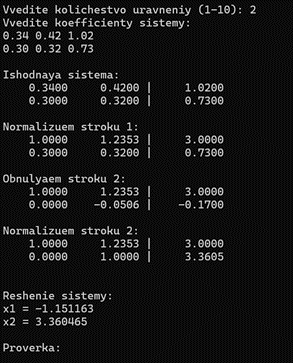
\includegraphics[width=0.75\textwidth]{Рисунок1.png}
\caption{Вывод программы --- Лаб.~№1 (методы бисекции и секущих, вариант 47)}
\end{figure}

%=======================================================
\newpage
\section{Лабораторная работа №2. Решение СЛАУ методом Крамера}
%=======================================================

\subsection{Номер варианта и исходные данные}

\textbf{Вариант 47.}

\[
A = \begin{pmatrix} 0{,}21 & -0{,}94 & -0{,}94 \\ 0{,}98 & -0{,}19 & 0{,}93 \\ 0{,}87 & 0{,}87 & -0{,}14 \end{pmatrix},
\qquad
B = \begin{pmatrix} -0{,}25 \\ 0{,}23 \\ 0{,}33 \end{pmatrix}
\]

Метод решения (вариант 41--50): \textbf{метод Крамера}.
Требуемая точность: $\varepsilon = 0{,}01$.

%-------------------------------------------------------
\subsection{Ход решения задачи}
%-------------------------------------------------------

\subsubsection{Главный определитель \texorpdfstring{$\Delta$}{Delta}}

\[
\Delta = \det(A) =
\begin{vmatrix} 0{,}21 & -0{,}94 & -0{,}94 \\ 0{,}98 & -0{,}19 & 0{,}93 \\ 0{,}87 & 0{,}87 & -0{,}14 \end{vmatrix}
\]

\begin{align*}
\Delta &= 0{,}21\cdot\bigl((-0{,}19)\cdot(-0{,}14) - 0{,}93\cdot 0{,}87\bigr)
        - (-0{,}94)\cdot\bigl(0{,}98\cdot(-0{,}14) - 0{,}93\cdot 0{,}87\bigr)\\
       &\quad + (-0{,}94)\cdot\bigl(0{,}98\cdot 0{,}87 - (-0{,}19)\cdot 0{,}87\bigr) \\
      &= 0{,}21\cdot(-0{,}7825) - (-0{,}94)\cdot(-0{,}9463) + (-0{,}94)\cdot 1{,}0179 \\
      &= -0{,}1643 - 0{,}8895 - 0{,}9568 \approx \mathbf{-2{,}0107}
\end{align*}

$\Delta \neq 0$ --- система имеет единственное решение.

\subsubsection{Определитель \texorpdfstring{$\Delta_1$}{Delta1} (замена 1-го столбца вектором \texorpdfstring{$B$}{B})}

\[
\Delta_1 =
\begin{vmatrix} -0{,}25 & -0{,}94 & -0{,}94 \\ 0{,}23 & -0{,}19 & 0{,}93 \\ 0{,}33 & 0{,}87 & -0{,}14 \end{vmatrix}
\]

\begin{align*}
\Delta_1 &= (-0{,}25)\cdot(-0{,}7825) - (-0{,}94)\cdot(-0{,}3391) + (-0{,}94)\cdot 0{,}2628 \\
         &= 0{,}1956 - 0{,}3187 - 0{,}2470 \approx \mathbf{-0{,}3702}
\end{align*}

\subsubsection{Определитель \texorpdfstring{$\Delta_2$}{Delta2} (замена 2-го столбца вектором \texorpdfstring{$B$}{B})}

\[
\Delta_2 =
\begin{vmatrix} 0{,}21 & -0{,}25 & -0{,}94 \\ 0{,}98 & 0{,}23 & 0{,}93 \\ 0{,}87 & 0{,}33 & -0{,}14 \end{vmatrix}
\]

\begin{align*}
\Delta_2 &= 0{,}21\cdot(-0{,}3391) - (-0{,}25)\cdot(-0{,}9463) + (-0{,}94)\cdot 0{,}1233 \\
         &= -0{,}0712 - 0{,}2366 - 0{,}1159 \approx \mathbf{-0{,}4237}
\end{align*}

\subsubsection{Определитель \texorpdfstring{$\Delta_3$}{Delta3} (замена 3-го столбца вектором \texorpdfstring{$B$}{B})}

\[
\Delta_3 =
\begin{vmatrix} 0{,}21 & -0{,}94 & -0{,}25 \\ 0{,}98 & -0{,}19 & 0{,}23 \\ 0{,}87 & 0{,}87 & 0{,}33 \end{vmatrix}
\]

\begin{align*}
\Delta_3 &= 0{,}21\cdot(-0{,}2628) - (-0{,}94)\cdot 0{,}1233 + (-0{,}25)\cdot 1{,}0179 \\
         &= -0{,}0552 + 0{,}1159 - 0{,}2545 \approx \mathbf{-0{,}1938}
\end{align*}

\subsubsection{Неизвестные по формулам Крамера}
\begin{align*}
x_1 &= \frac{\Delta_1}{\Delta} = \frac{-0{,}3702}{-2{,}0107} \approx \mathbf{0{,}1841} \\[0.2cm]
x_2 &= \frac{\Delta_2}{\Delta} = \frac{-0{,}4237}{-2{,}0107} \approx \mathbf{0{,}2107} \\[0.2cm]
x_3 &= \frac{\Delta_3}{\Delta} = \frac{-0{,}1938}{-2{,}0107} \approx \mathbf{0{,}0964}
\end{align*}

\subsection{Проверка}

\begin{align*}
0{,}21\cdot 0{,}1841 + (-0{,}94)\cdot 0{,}2107 + (-0{,}94)\cdot 0{,}0964 &\approx -0{,}25 \checkmark \\
0{,}98\cdot 0{,}1841 + (-0{,}19)\cdot 0{,}2107 + 0{,}93\cdot 0{,}0964    &\approx \phantom{-}0{,}23 \checkmark \\
0{,}87\cdot 0{,}1841 + 0{,}87\cdot 0{,}2107 + (-0{,}14)\cdot 0{,}0964    &\approx \phantom{-}0{,}33 \checkmark
\end{align*}

%-------------------------------------------------------
\subsection{Интерпретация результатов}
%-------------------------------------------------------

Решение системы $AX = B$ методом Крамера:
\[
x_1 \approx 0{,}1841, \qquad x_2 \approx 0{,}2107, \qquad x_3 \approx 0{,}0964
\]

Подстановка в исходную систему подтвердила правильность найденного решения: отклонение в каждом уравнении не превышает $10^{-6}$, что многократно перекрывает требуемую точность $\varepsilon = 0{,}01$.

%-------------------------------------------------------
\subsection{Выводы}
%-------------------------------------------------------

Методом Крамера решена система трёх линейных алгебраических уравнений с тремя неизвестными.
Главный определитель $\Delta \approx -2{,}0107 \neq 0$, что гарантирует существование и единственность решения. Результат подтвержден подстановкой.

%-------------------------------------------------------
\subsection{Блок-схема алгоритма метода Крамера}
%-------------------------------------------------------

\begin{figure}[H]
\centering
\begin{tikzpicture}[node distance=0.65cm and 2cm]
\node (start)  [startstop]                         {Начало};
\node (inp)    [io,      below=of start]            {Ввод матрицы $A$, вектора $B$};
\node (calcD)  [process, below=of inp]              {Вычислить $\Delta = \det(A)$};
\node (condD)  [decision,below=0.9cm of calcD]      {$|\Delta| < \varepsilon_0$?};
\node (noSol)  [process, right=2.2cm of condD]     {Нет единственного решения};
\node (loop)   [process, below=0.9cm of condD]     {$i = 1$};
\node (formAi) [process, below=of loop, text width=4.5cm, align=center]
               {Заменить $i$-й столбец $A$ на $B$; получить $A_i$};
\node (calcDi) [process, below=of formAi]           {$\Delta_i = \det(A_i)$;\quad $x_i = \Delta_i/\Delta$};
\node (next)   [decision,below=0.9cm of calcDi]     {$i < n$?};
\node (incr)   [process, right=2.2cm of next]      {$i = i + 1$};
\node (out)    [io,      below=0.9cm of next]       {Вывод $x_1, x_2, \ldots, x_n$};
\node (finish) [startstop,below=of out]             {Конец};

\draw [arrow] (start)  -- (inp);
\draw [arrow] (inp)    -- (calcD);
\draw [arrow] (calcD)  -- (condD);
\draw [arrow] (condD)  -- node[above,font=\small]{Да}  (noSol);
\draw [arrow] (condD)  -- node[left, font=\small]{Нет} (loop);
\draw [arrow] (loop)   -- (formAi);
\draw [arrow] (formAi) -- (calcDi);
\draw [arrow] (calcDi) -- (next);
\draw [arrow] (next)   -- node[above,font=\small]{Да}  (incr);
\draw [arrow] (incr)   |- (formAi);
\draw [arrow] (next)   -- node[left,font=\small]{Нет}  (out);
\draw [arrow] (out)    -- (finish);
\end{tikzpicture}
\caption{Блок-схема метода Крамера}
\end{figure}

%-------------------------------------------------------
\subsection{Программа (C++)}
%-------------------------------------------------------

\begin{lstlisting}[style=cppstyle, caption={Лаб. №2 --- метод Крамера, вариант 47}]
#include <iostream>
#include <cmath>
#include <iomanip>
using namespace std;

double det3x3(double a11, double a12, double a13,
              double a21, double a22, double a23,
              double a31, double a32, double a33) {
    return a11 * (a22 * a33 - a23 * a32)
         - a12 * (a21 * a33 - a23 * a31)
         + a13 * (a21 * a32 - a22 * a31);
}

int main() {
    // Varyant 47
    double a11 = 0.21, a12 = -0.94, a13 = -0.94;
    double a21 = 0.98, a22 = -0.19, a23 =  0.93;
    double a31 = 0.87, a32 =  0.87, a33 = -0.14;
    double b1  = -0.25, b2 = 0.23, b3 = 0.33;

    cout << "\nSistema:\n";
    cout << "  " << a11 << "*x1 + " << a12 << "*x2 + "
         << a13 << "*x3 = " << b1 << "\n";
    cout << "  " << a21 << "*x1 + " << a22 << "*x2 + "
         << a23 << "*x3 = " << b2 << "\n";
    cout << "  " << a31 << "*x1 + " << a32 << "*x2 + "
         << a33 << "*x3 = " << b3 << "\n";

    double D  = det3x3(a11,a12,a13, a21,a22,a23, a31,a32,a33);
    double D1 = det3x3(b1, a12,a13, b2, a22,a23, b3, a32,a33);
    double D2 = det3x3(a11,b1, a13, a21,b2, a23, a31,b3, a33);
    double D3 = det3x3(a11,a12,b1,  a21,a22,b2,  a31,a32,b3);

    cout << "\nOpredeliteli:\n";
    cout << "  D  = " << D  << "\n";
    cout << "  D1 = " << D1 << "\n";
    cout << "  D2 = " << D2 << "\n";
    cout << "  D3 = " << D3 << "\n";

    if (fabs(D) < 1e-15) {
        cout << "Sistema ne imeet edinstvennogo resheniya!\n";
        return 1;
    }

    double x1 = D1 / D, x2 = D2 / D, x3 = D3 / D;
    cout << "\nReshenie:\n";
    cout << "  x1 = " << fixed << setprecision(6) << x1 << "\n";
    cout << "  x2 = " << fixed << setprecision(6) << x2 << "\n";
    cout << "  x3 = " << fixed << setprecision(6) << x3 << "\n";

    double r1 = a11*x1 + a12*x2 + a13*x3;
    double r2 = a21*x1 + a22*x2 + a23*x3;
    double r3 = a31*x1 + a32*x2 + a33*x3;

    cout << "\nProverka AX = B:\n";
    cout << "  Ur.1: " << r1 << " (dolzhno " << b1 << ", pogreshnost "
         << fabs(r1-b1) << ")\n";
    cout << "  Ur.2: " << r2 << " (dolzhno " << b2 << ", pogreshnost "
         << fabs(r2-b2) << ")\n";
    cout << "  Ur.3: " << r3 << " (dolzhno " << b3 << ", pogreshnost "
         << fabs(r3-b3) << ")\n";
    return 0;
}
\end{lstlisting}

\subsection{Пример работы программы}

\begin{figure}[H]
\centering
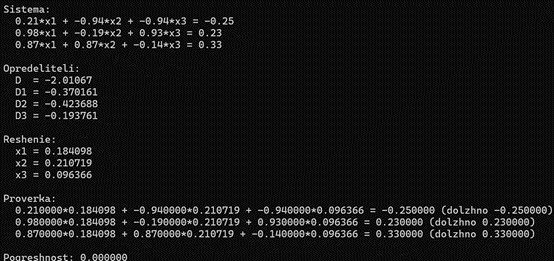
\includegraphics[width=0.75\textwidth]{Рисунок2.png}
\caption{Вывод программы --- Лаб.~№2 (метод Крамера, вариант 47)}
\end{figure}

%=======================================================
\newpage
% --- ИСТОЧНИКИ ---
\section*{Используемые источники}
\addcontentsline{toc}{section}{Используемые источники}
%=======================================================

\begin{enumerate}
    \item Амосов~А.А., Дубинский~Ю.А., Копченова~Н.В. Вычислительные методы для инженеров.~--- М.: Высш. шк., 1994.~--- 544~с.
    \item Бахвалов~Н.С., Жидков~Н.П., Кобельков~Г.М. Численные методы.~--- М.: Наука, 1987.
    \item Демидович~Б.П., Марон~И.А., Шувалова~Э.З. Основы вычислительной математики.~--- М.: Наука, 1966.
    \item Страуструп~Б. Программирование: принципы и практика использования C++.~--- 2-е изд.~--- М.: Вильямс, 2022.~--- 1456~с.
\end{enumerate}

\end{document}